\documentclass{article}
\usepackage[utf8]{inputenc}
\UseRawInputEncoding
\usepackage{graphicx, booktabs}
\title{\textbf{Deep Learning Lab}\\ Assignment 3}
\author{Felix Boelter}
\date{\today}

\usepackage{listings}
\lstset{
basicstyle=\small\ttfamily,
columns=flexible,
breaklines=true
}
\begin{document}

\maketitle

\section{Language Modeling with RNNs}
\subsection{Loading Into A String}
The raw book was loaded into a string using the requests python library, it was then written into a text file, which can be used later to retrieve the text.
\subsection{Properties of data}
I created a counter method which goes through the whole text, the results are:
\begin{center}
Word Count:  5033\\
Line Count:  5033\\
Char Count (no white spaces):  138881\\
Sentence Count:  1880\\
\end{center}
\subsection{Splitting data into Chunks}
The data was split into chunks with a BPTT span of 256 and a batch size of 64. Thus we get 11 chunks (with whitespaces). For the train field, I use Field from torchtext, I tokenize every character with init tokens being set to $<sos>$ and eos tokens being set to $<eos>$.\\ The train dataset is being created by the LanguageModelingDataset, which takes the path to the string, which was created in 1.1 and the text field which is the train field. We can then build the vocab using the train field, which comes out to be of length 108.\\ When splitting the data into chunks I use the BPTTIterator from torchtext, which takes in the dataset, a batch size and a BPTT span.
\subsection{LSTM Language Model}
For the network, I am using an Embedding layer, an LSTM layer and a Linear layer. When creating the LSTMModel it takes in an embedding dimension, a hidden size, a batch size, a vocabulary size and the number of recurrent layers.
\subsection{Greedy Decoding}
\begin{enumerate}
    \item We tokenize the string and convert them to an integer array.
    \item We pass the initial input through our model and send the output into a Softmax which can then be sent through an argmax.
    \item We loop over the length of the sequence that we want to create, and send the argmax in the position of the last character of the string to the model.
    \item The model creates another output that has to be sent through a Softmax and then through an argmax, then we convert the integer created from the argmax into a character, which is appended to a list.
    \item This integer created from the argmax is sent back to the model and the loop is repeated.
    \item Finally we join our finished generated sequence and get one single string which is returned.
\end{enumerate}
\subsection{Random Sampling}
\begin{enumerate}
    \item We tokenize the string and convert them to an integer array.
    \item We pass the initial input through our model and send the output into a Softmax which can then be sent through a multinomial.
    \item We loop over the length of the sequence that we want to create, and send the multinomial with 1 random sample in every row of the tensor, in the position of the last character of the string to the model.
    \item The model creates another output that has to sent through a Softmax and then through a multinomial, then we convert the integer created from the multinomial into a character, which is appended to a list.
    \item This integer created from the multinomial is sent back to the model and the loop is repeated.
    \item Finally we join our finished generated sequence and get one single string which is returned.
\end{enumerate}
\clearpage
\subsection{Creating Training}
The model was trained using Adam optimizer and the CrossEntropyLoss function. The hidden states were reset every epoch and the model was trained on batches. The hidden state was also detached from the history so the loss didn't backpropagate through the batches. Every epoch the model was evaluated on sentences/titles from the training file, using greedy and random sampling decoding. The perplexity of the model on the training data was also evaluated.
\subsection{Training the Model}
\begin{table}[ht]
\centering
\resizebox{\columnwidth}{!}{%
\begin{tabular}{@{}ccccccc@{}}
\toprule
\textbf{Epochs} & \textbf{Batch Size} & \textbf{BPTT Span} & \textbf{Learning Rate} & \textbf{Embedding Size} & \textbf{Hidden Size} & \textbf{Layers} \\ \midrule
100 & 64 & 256 & $10^{-3}$ & 1024 & 1024 & 2 \\ \bottomrule
\end{tabular}%
}
\caption{The best hyperparameters I found to make the model converge to less than 1.03 perplexity.}
\label{tab:hyper}
\end{table}
\begin{figure}[ht]
    \begin{minipage}[c]{.60\textwidth}
			\centering
			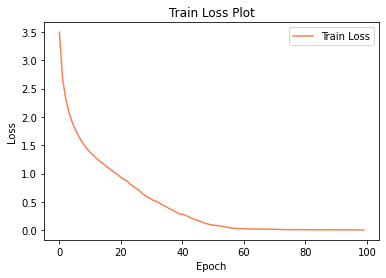
\includegraphics[width=\linewidth]{images/train_loss.png}
			\caption{Evolution of Training Loss}
		\end{minipage}
		~
		\begin{minipage}[c]{.60\textwidth}
			\centering
			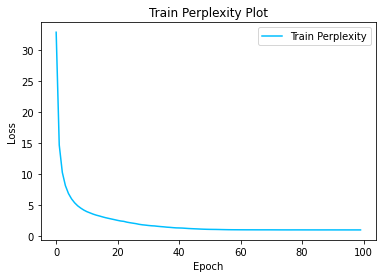
\includegraphics[width=\linewidth]{images/perplexity.png}
			\caption{Evolution of Training Perplexity}
		\end{minipage}
\end{figure}
In the first epochs, the Greedy as well as the Random decoding create output which doesn't make sense.
\begin{lstlisting}
Greedy decoding
Sample prompt: Dogs like best to | generated text: the the the the the the the the 
the the the the the the the the the the the the the the the the the 
Random decoding
Sample prompt: Dogs like best to | generated text: wof wi Fourd inmt,,rypen ” ukppet ou Ghe og to oy ranc.<eos>h hotoiths<eos>1OigB bser.<eos><eos>W<eos><eos>E<eos>Ihytun
\end{lstlisting}
At epoch 50 the model starts to make more sense, the greedy decoding algorithm looks better here as the random decoding looks like it doesn't understand the prompt at all.
\begin{lstlisting}
Greedy decoding
Sample prompt: Dogs like best to | generated text: eat at home, and<eos>
he stretched him so much to me.<eos><eos>"There is nothing I hate like a bird," said the Bo
Random decoding
Sample prompt: Dogs like best to | generated text: end of the<eos>difficulties 
in handing down litely hope,<eos>compristributing or creating derivative works b

\end{lstlisting}
At epoch 100 the model gets the correct training text from the dataset. The greedy aswell as the random decoding get the same result.
\begin{lstlisting}
Greedy decoding
Sample prompt: Dogs like best to | generated text: eat at home, and he<eos>complained 
bitterly.<eos><eos>The Mule, meeting him soon after, knew him and called out:
Random decoding
Sample prompt: Dogs like best to | generated text: eat at home, and he<eos>complained 
bitterly.<eos><eos>The Mule, meeting him soon after, knew him and called out:

\end{lstlisting}
\clearpage
\subsection{A few different Prompts}
\textbf{Greedy Decoding}\\\\
\emph{A title in the book}
\begin{lstlisting}
Sample prompt: THE FOX AND THE LION | generated text: <eos><eos>THE first time the Fox saw the Lion, he was ready to die of fear. The<eos>second time he took courage and could even bear to look upon him. The<eos>third time he had the impudence to come up to him, to salute him, and<eos>to enter into familiar conversation with him.<eos><eos><eos><eos><eos>THE DOG AND HIS SHADOW<eos><eos><eos>A DOG had sto
\end{lstlisting}
\emph{A title in similar style}
\begin{lstlisting}
Sample prompt: THE TURTLE AND THE BIRD | generated text: <eos><eos><eos>A WISE Swallow, seeing a man sow seed in a field, went behind him and<eos>picked up one of the seeds to see what it was.<eos><eos>She found that it was flax. “When this flax has grown,” she said to<eos>herself, “the man will make it into linen thread and use it to make<eos>nets for catching us Birds.”<eos><eos>So she went t
\end{lstlisting}
\emph{Some texts in similar style}
\begin{lstlisting}
Sample prompt: Back in my day | generated text:  The Iniman so was my obtain it is outright to strike<eos>himself in the daytime but hides in lonely! how you can make a dinner of me then, or sell me<eos>for a good price.”<eos><eos>“Ah!” said the Fisherman, “it is true you are small, but I have you<eos>safely now. If she should go by, I can easily enough<eos>catch up.”<eos><eos>
\end{lstlisting}
\emph{Anything Interesting}
\begin{lstlisting}
Sample prompt: Dallmayr to go | generated text: that used the spirit to fight or remove the full Project Gutenberg-tm<eos>License terms from this work, or any files containing a part of this<eos>work or any other work associated with Project Gutenberg-tm.<eos><eos>1.E.5. Do not copy, display, perform, distribute or redistribute this<eos>electronic work, or any part 
Sample prompt: Covid-19 is | generated text: not in hand<eos>came at length to her. Not one of them could she<eos>persuade to help her pick up the seeds which the farmer had sown.<eos><eos>By and by the flax sprang up, and the Swallow tried again to persuade<eos>the Birds to pull the young flax before it grew large. But they all<eos>made fun of her caution and let th
\end{lstlisting}
\textbf{Random Decoding}\\\\
\emph{A title in the book}
\begin{lstlisting}
Sample prompt: THE FOX AND THE LION | generated text: <eos><eos>THE first time the Fox saw the Lion, he was ready to die of fear. The<eos>second time he took courage and could even bear to look upon him. The<eos>third time he had the impudence to come up to him, to salute him, and<eos>to enter into familiar conversation with him.<eos><eos><eos><eos><eos>THE DOG AND HIS SHADOW<eos><eos><eos>A DOG had sto
\end{lstlisting}
\emph{A title in similar style}
\begin{lstlisting}
Sample prompt: THE TURTLE AND THE BIRD | generated text: <eos><eos><eos>A WISE Swallow, seeing a man sow seed in a field, went behind him and<eos>picked up one of the seeds to see what it was.<eos><eos>She found that it was flax. “When this flax has grown,” she said to<eos>herself, “the man will make it into linen thread and use it to make<eos>nets for catching us Birds.”<eos><eos>So she went t
Some texts in similar style
Sample prompt: Back in my day | generated text: .<eos><eos>The Wolf stopped and set to work to rescue the Fox. Its method was a<eos>simple one—it bit the tail clean off.<eos><eos>So our foolish friend went home tailless, but rejoicing that its skin<eos>was still on its back.<eos><eos><eos><eos><eos>THE INQUISITIVE MAN<eos><eos><eos>“GOOD day, dear friend; where do you come from?”<eos><eos>“From the Museum, wh
\end{lstlisting}
\emph{Anything Interesting}
\begin{lstlisting}
Sample prompt: Dallmayr to go | generated text: that us it mayself fell be.<eos><eos>The Hare agreed, a course was arranged, and away they started together.<eos><eos>They weren’t quite as to pleas, the United States and most<eos>other parts of the world at no cost and with almost no restrictions<eos>whatsoever.  You may copy it, give it away or re-use it under the terms
Sample prompt: Covid-19 is | generated text: not it provided to you 'AS-IS', WITH NO<eos>OTHER WARRANTIES OF ANY KIND, EXPRESS OR IMPLIED, INCLUDING BUT NOT<eos>LIMITED TO WARRANTIES OF MERCHANTABILITY OR FITNESS FOR ANY PURPOSE.<eos><eos>1.F.5. Some states do not allow disclaimers of certain implied<eos>warranties or the exclusion or limitation of certain types
\end{lstlisting}
\clearpage
\subsection{Comparing Greedy and Random Sampling Decoding}
The random sampling decoding text actually generates much more interesting text. As it is random, it can create very interesting text if you load the prompt another time, the greedy decoding on the other hand generates text that is always the same, since it has the highest probability. Since the text generated can change on every run, in the random sampling, I think that it is much better since you can run it till the text generated makes a lot more sense.
\subsection{Quality of the generated text}
The output is meaningful however there are cases where the predictor generates the same words and sentences multiple times. The predictor correctly creates capitilization after a full stop it also capitilizes nouns correctly. Moreover, it also correctly predicts when to use commas.\\
When given a title of a fable it correctly predicts the text which is found in the book up to around 100 characters until it tries to create something else. When given a prompt title which is not in the book, it correctly predicts new text in the style of a fable.
\clearpage
\subsection{Results for 5 Prompts that are interesting}
\begin{lstlisting}

Sample prompt: The Fox | generated text:  and their god,<eos>to the Dog could not be trusted,<eos>and at the same time to punish the Dog himself, the master would<eos>sometimes hang a bell about his neck and compel him to drag a heavy<eos>clog, which he firmly attached to his collar by a chain.<eos><eos>For a time the Dog hung his head; but seeing that his bell and clog<eos>brought him into notice, he grew proud of them, and ran about the<eos>market place to display them and attract attention to himself. He even<eos>went so far as to give himself airs with the other dogs

Sample prompt: A plastic bottle | generated text:  with me<eos>for being too fond of honey; yet all use father’s<eos>had for whis long enemy, the Cock sore of general creature<eos>strutting at their goal.<eos><eos>Those who are very quick are apt to be too sure. Slow and steady often<eos>wins the race.<eos><eos><eos><eos><eos>THE ARAB AND HIS CAMEL<eos><eos><eos>AS AN Arab sat in his tent one cold night, he saw the curtain gently<eos>lifted, and the face of his Camel looking in.<eos><eos>“What is it?” he asked kindly.<eos><eos>“It is cold, master,” said the Camel; “suffer me, I pray thee, to hold<eos>my head within the ten

Sample prompt:   | generated text: topped to look at them.<eos><eos>“What a foolish creature you were, to hatch those eggs!” said the<eos>Swallow. “Don’t you know that as soon as the little snakes grow big<eos>enough, they will bite some one—probably _you_ first of all?”<eos><eos>“Then,” said the Hen, as she stood on one leg and looked at the ugly<eos>little snakes, first with one eye and then with the other, “you think<eos>I have done more harm than good?”<eos><eos>“I certainly do,” said the Swallow, as she flew away. “Good judgment is<eos>better than thoughtless kindness


Sample prompt: A FOX was once caught in a trap by his | generated text: tail. He succeeded in getting<eos>away, but was forced to leave his “brush” behind. He soon realized that<eos>his life would be a burden, for the handing down day.<eos>The Mouse showed the Frog his nest and everything he could think<eos>out they were untied: “I shall get that way, you would never reach half its size.” Vexed that her child should disparance<eos>opproached warmraid was hard for the preceding small be foes. What<eos>a little waiting is load warming, the Eagle swam a good price.

Sample prompt: <eos> | generated text: to come and live<eos>with me; I have plenty of food and water, and nothing to disturb me;<eos>and it is so pleasant in my pond. Now here there is very little food,<eos>and not much water, and the road passes through your pool, so that you<eos>must always be afraid of passers-by.”<eos><eos>“Thank you,” said the other Frog; “you are very kind, but I am quite<eos>content here. There is water enough; those who pass never trouble me;<eos>and as to food, I had a good dinner day before yesterday. I am used to<eos>this place, you know, and do not like change. If you are outside the United States,<eos>check the laws of your country in additi

Sample prompt: <eos> | generated text: to come and live<eos>with me; I have plenty of food and water, and nothing to disturb me;<eos>and it is so pleasant in my pond. Now here there is very little food,<eos>and not much water, and the road passes through your pool, so that you<eos>must always be afraid of passers-by.”<eos><eos>“Thank you,” said the other Frog; “you are very kind, but I am quite<eos>content here. There is water enough; those who pass never trouble me;<eos>and as to food, I had a good dinner day before yesterday. I am used to<eos>this place, you know, and do not like change. If you are outside the<eos>United States, you'll have to check the laws of the cou


\end{lstlisting}
The last prompt was the most interesting, since I started with a $<eos>$, it actually generated the same text in the greedy decoder and the random sampling decoder. The last part about the United States was actually better written in the greedy decoder than in the random sampling decoder.
\subsection{Bonus: Donald Trump Rally speeches}
I took three rally speeches as my input, these were the counts for my input:
\begin{center}
    Word Count:  1785\\
    Line Count:  1785\\
    Character Count:  212573\\
    Sentence Count:  4852\\
    Vocabulary Count:  86\\
\end{center}
The hyperparameter settings were the same as in the last model, as they worked pretty well again:
\begin{table}[ht]
\centering
\resizebox{\columnwidth}{!}{%
\begin{tabular}{@{}ccccccc@{}}
\toprule
\textbf{Epochs} & \textbf{Batch Size} & \textbf{BPTT Span} & \textbf{Learning Rate} & \textbf{Embedding Size} & \textbf{Hidden Size} & \textbf{Layers} \\ \midrule
100 & 64 & 256 & $10^{-3}$ & 1024 & 1024 & 2 \\ \bottomrule
\end{tabular}%
}
\caption{Model hyperparameters}
\label{tab:hyper}
\end{table}
\textbf{Greedy Decoding}
\begin{lstlisting}
Sample prompt: Thank You | generated text:  Thank you very much. We appreciate it. Next year will be the greatest economic year in the history of our country. That’s where we’re heading. Super V. Joe Biden doesn’t even respect you enough to have a China in there because I like to be accurate. But, but he said, “Sir, you have tested positive 

Sample prompt: Good | generated text: late the next do on, really not a politician for one very specific reason because we’re doing a job in the history of our country in the first three and a half years, nobody has done what we, what we, and this administration has been able to do with regulations, with taxes, with rebuilding our milit

Sample prompt: China | generated text:  This is not the crowd of a second place finisher. Do you agree with that? No. No. This is our crowd, all together. We’re in this together and we’re doing it together. As long as I’m President, we will remain the number one producer of oil and natural gas anywhere on this planet. And for the first t

Sample prompt: We have to | generated text: now finish the progress. A vote for Biden is a vote to hand the keys of government over to people who don’t like you, don’t respect you, and who want to rob your children of their American dream. We have a great American dream. We’re not going to let it happen. We’re not going to let that happen. We
\end{lstlisting}
\textbf{Random Decoding}
\begin{lstlisting}
Sample prompt: Thank You | generated text:  Thank you very much. Everything good? You’re doing great. Thank you, Bill.<eos><eos>Donald Trump: (02:20:49)<eos>Congressional candidate, Peter Meijer. Peter, where’s Peter? Where’s Peter? Peter, you don’t have a good location. What happened to Peter? Peter’s here someplace and I hear he’s doing great.<eos><eos>Donald
Sample prompt: Good | generated text: job. Unbelievable. Unbelievable. Is that better now?<eos><eos>Audience: (05:12)<eos>Yes!<eos><eos>President Donald J. Trump: (50:20)<eos>Thank you, everybody. It’s a great honor to be with you. I really did, during the Kenosha disaster, I really got to be friendly with a lot of people up here. Long before that because we’v
Sample prompt: China | generated text:  Preaty This is not for a lifetime. It’s only for four months. Immunity is only now for four months.” They brought it down, right? It was always going to be for a lifetime, now it’s four months. So what are you going to do? What are you going to do? It’s one of those things, but I think our country 
Sample prompt: We have to | generated text: make this… You have to get out there on Monday, Tuesday, Sunday, I don’t care, today. You have to get out there and vote. Most of you are going to vote because you believe in voting, like I do. I just left. I just voted two days ago. I voted. I went to a booth, and they actually asked me, “Sir, may 

Sample prompt:   | generated text: ant your children to be safe, if you want your values to be respected, if you want to be just treated with dignity and respect, then I am asking you tomorrow to go out and vote for your all time favorite President, because we still have work to do.<eos><eos>Speaker 1: (35:07)<eos>Four more years! Four more years! Four more years!<eos><eos>President Donald J. Trump: (50:22)<eos>Thank you, everybody. It’s a great honor to be with you. I really did, during the Kenosha disaster, I really got to be friendly with a lot of people up here. Long before that because we’ve had so many different people that we deal with. You have great people, we’re going to introduce you to a few of them, but you have great people here. But I really got to know you during that problem. That potential crisis that we put out very, very swiftly once we got called and it’s great. You’re great people. You built the country, you’re great people. Joe Biden, and as I said, he ran the H1NI, he called it N1H1, he couldn’t get it right. He still d
Sample prompt:   | generated text: hey go, “Oh, hello.” Can you actually hear this? Can you hear this?<eos><eos>President Donald J. Trump: (20:46)<eos>Because this is the worst microphone I’ve ever used in my life. Can you actually hear me over there? They can. In the back, all the way back. That’s good. Thank you. I can’t believe it. It sounds terrible to me. It doesn’t sound great, right? To me, it doesn’t sound great. It’s all right. Good. You know what? Keep saying it. That Bill, he says, “Don’t pay him. Don’t pay him.” Did you hear that, Johnny? Don’t pay the damn bill, would you please? A piece of garbage they gave me. It’s not even the first rate mic. The good one, it’s put to rest. We put it the rest. The good one, we put the rest. All right, don’t pay him. But as President, I will ensure peace through strength. And that’s what we have now, with what we have. We will end surprise medical billing, require price transparency, which goes into effect on January 1st, bigger than healthcare. Lower drudg positive development for n
Something not in the text
Random Decoding
Sample prompt: Birds fly high | generated text: st was Vice President, we actually saw a steady assault on our first freedom, the freedom of religion. The last administration used the power of the federal government to erode the conscience rights of doctors and nurses in religious charities. They even hauled a group of nuns into federal court to 
Greedy Decoding

Sample prompt: Birds fly high | generated text: st was a little bit of a nod, they say the president led them on. Now I don’t have to leave you on. Even a little nod, they say the president said, right? They asked me that question are crazy 60 Minutes. Wasn’t she rude? She just kept asking me questions. And then they interviewed sleepy Joe, and i
\end{lstlisting}
The model is actually creating the rally speeches pretty well, when given a white space as input it can actually create very nice text that is in the style of a Donald Trump speech.
\clearpage
\subsubsection{5 Interesting Prompts}
\begin{lstlisting}
Greedy Decoding

Sample prompt: <eos> | generated text: plan to find somebody so badly. But it’s never been said before to the best of anyone’s knowledge.<eos><eos>Donald Trump: (01:39:03)<eos>… so badly, but it’s never been said before to the best of anyone’s knowledge.<eos><eos>Donald Trump: (01:39:03)<eos>… so badly, but it’s never been said before to the best of anyone’s knowledge.<eos><eos>Donald Trump: (01:39:03)<eos>… so badly, but it’s never been said before to the best of anyone’s knowledge.<eos><eos>Donald Trump: (01:39:03)<eos>… so badly, but it’s never been said before to the best of anyone’s knowledge.<eos><eos>Donald Trump: (01:39:03)<eos>… so badly, but it’s never been said before to the best

Random Decoding

Sample prompt: <eos> | generated text: plans, like youw out and vote, like laway, which was unscheduled. So I got a call from Ronna, the whole group, and they said, “Could you go back?” We got here at 12:00 in the evening, I started speaking at 12:30, now election day, I’ll never forget it. We had 32,000 people, almost as many as we have tonight. And I said to my team, “We have to … This is it.” We’ve done five, but actually six, because we ended up last night around 2:00 in the morning in Miami, so we can say that includes this … So that would be six. We’ve done six of these big, and every one was just a lot of people. And you kno
\end{lstlisting}
This looks very interesting, as the greedy decoding keeps on repeating the same sentence when given a $<eos>$ as a prompt. The random decoding makes a lot more sense and it really seems like its one of Donald Trumps ramblings when he speaks in the rallies.
\begin{lstlisting}
Greedy Decoding

Sample prompt: Money | generated text:  this is a poll. See, this is a poll. When you draw crowds like this. This is not the crowd of somebody that’s going to lose the state of Michigan. This is not. This is not. And look at this crowd. You can’t even see the end of it. You can’t. This is not the crowd of a second place finisher. Do you agree with that? No. No. This is our crowd, all together. We’re in this together and we’re doing it together. As long as I’m President, we will remain the number one producer of oil and natural gas anywhere on this planet. And for the first time, we are energy independent. You never heard that term 

Random Decoding

Sample prompt: Money | generated text:  this is a had vayer anybody, but they don’t want… And I keep saying, “Well, how are we doing with Antifa, the anarchists?” This Election Day, you must stop the anti-American radicals by delivering Joe Biden and the far left a thundering defeat at the ballot box on November 3rd. It’s got to be a big one, we’ve got to win big. And we’re going to win big, I watching them and they’re getting… Like three weeks ago, I don’t know, they were doing these fake polls and they felt very good. And then a week ago they were feeling okay, they’re not feeling so good right now. They’re saying, “These are not

Greedy Decoding

Sample prompt: Covid 19 | generated text: 5 million jobs in the last five months alone, which is another record. That’s another big record. We’ve never hired that many people that fast. While foreign nations are in a free fall, we’re creating an economic powerhouse unrivaled anywhere in the world. A recent Gallup Poll found that 56% of Americans say they are better off today than they were four years ago under Obama and Biden. And if Biden and Kamala … You don’t have to say it “Kamala.” “Kamala.” If Biden and Kamala Harris, who’s further left by far than crazy Bernie Sanders, right, he’s considered a strict conservative compared to he

Random Decoding

Sample prompt: Covid 19 | generated text: 5 never heard that before. You know, I’ve covered politicians. I’ve been friends with politicians. I’ve been enemies also, but I’ve never seen somebody saying we will raise your taxes. They want to give you the largest tax increase in the history of our country, and we can’t let that happen. We can’t let that happen.<eos><eos>President Donald J. Trump: (07:42)<eos>So get out and vote. Tomorrow will be, I think, will be the most important election in the history of our country, and I never thought I’d say that. I never thought I’d say it. So get out and vote. Sleepy Joe Biden will raise your taxes $4 trill

Greedy Decoding

Sample prompt: model.eval() | generated text:  They don’t want to hear it. We’re making that turn. You know that right? We’re going to have the vaccine anyway with, or without it, we’re making the turn. Normal life will fully resume. That’s all we want. We want normal life, normal life, go back seven months, we’ll take normal life, greatest economy we ever had. We want normal life and next year will be the greatest economic year in the history of our country. That’s where we’re heading. Super V. Joe Biden doesn’t even respect you enough to have a China in there because I like to be accurate. But, but he said, “Sir, you have tested positiv

Random Decoding

Sample prompt: model.eval() | generated text: g and you have to come back. You have to come back. You have to come back. You have to come back.” I said, “Look, I’ll do it one more time.” Because Michigan, hadn’t been one in 36 years. I said, “Look, I’ll do it one more time. That’s it.” I came back. She said, “That’s it, sir. Don’t worry about it.” I left. Two days later, I get a one more phone call. “Sir, one more visit.” And we did. Do you know, Michigan was the last stop that I made. I made it in Grand Rapids, you know, they were doing these fake polls and they felt very good. And then a week ago they were feeling okay, they’re not feel

Greedy Decoding

Sample prompt: President Donald J. Trump:  | generated text: 01:14)<eos>Thank you very much and hello, Kenosha. It’s nice to be back. It’s nice to be back. We spent a little time with you, a little law and order. We brought law and order to Kenosha. Right? That’s what we want. And hello, Wisconsin. Big day, tomorrow, big, big day, big day. And I think we’re going to do very well in Wisconsin just like we did four years ago. And it’s an honor to be with you. Thank you.<eos><eos>Audience: (01:41)<eos>USA! USA! USA! USA!<eos><eos>President Donald J. Trump: (01:51)<eos>And this is a lot of people. This is a lot of people. See, you know what that means? That means we don’t have to pay 

Random Decoding

Sample prompt: President Donald J. Trump:  | generated text: 01:14)<eos>Thank you very much and hello, Kenosha. It’s nice to be back. It’s nice to be back. We spent a little time with you, a little law and order. We brought law and order to Kenosha. Right? That’s what we want. And hello, Wisconsin. Big day, tomorrow, big, big day, big day. And I think we’re going to do very well in Wisconsin just like we did four years ago. And it’s an honor to be with you. Thank you.<eos><eos>Audience: (01:41)<eos>USA! USA! USA! USA!<eos><eos>President Donald J. Trump: (01:51)<eos>And this is a lot of people. This is a lot of people. See, you know what that means? That means we don’t have to pay 

\end{lstlisting}
The most interesting one is where the prompt is 'President Donald J. Trump: ' because the Greedy and Random decoding both found the exact same sequence, which is created in the input text.
\clearpage
\section{Questions}
\subsection{Perplexity of a model that always predicts each character with equal probability?}
If there is a vocabulary size of 108 and we set the vocabulary size to $N$\\\\
$Perplexity = exp(-\frac{1}{N}\sum_{n=1}^{N}\log p(w_{n}|(w_{0}^{n-1}))$\\
$Perplexity = exp(-\frac{1}{N}\sum_{n=1}^{N}\log \frac{1}{N})$\\
$Perplexity = exp(-\log \frac{1}{N})$\\
$Perplexity = N$\\
Thus we get a Perplexity of 108 if our model always predicts each character with equal probability.
\subsection{Four other examples of sequence prediction problems that are not based on text}
\begin{enumerate}
    \item Time Forecasting, this is a sequence prediction problem as it looks at previous data and predicts new data, such as number of people in a specific train line during Summer.
    \item Product recommendation, when saving data of what people search or look at on the internet there can be recommendations that are made from such data.
    \item Prediction of stock market data using historical data or even more complex from news sources.
    \item Protein function prediction from amino-acid sequences.
\end{enumerate}
\subsection{Vanishing gradient problem}
When training an RNN, we have to minimize a loss function. When we update the hidden state we use the following equation:\\
\begin{center}
    $h^{(t)} = W^{T}h^{t-1}$
\end{center}
If $W^{T}$ is greater than 1 the hidden state will explode and go to $+\infty$ and it will vanish if it is less than 1 and go to $-\infty$.
\end{document}
